% =============================================================================
%  Household water treatment: fieldwork update for the PI
%  DIL Welcome Week · Session 5 exercise · A report that updates itself
%
%  This file never contains a typed result. Numbers come from
%  tables/numbers.tex, the table from tables/tab1-water-practices.tex and the
%  figure from figures/fig1-chlorination-village.png -- all written by
%  code/2-export-outputs.do. Rerun the code, push, pull, recompile.
% =============================================================================

\documentclass[11pt]{article}

\usepackage[margin=1in]{geometry}
\usepackage{booktabs}
\usepackage{graphicx}
\usepackage{threeparttable}
\usepackage[hidelinks]{hyperref}

% Every number quoted in the text: \nHH, \shareChlorine, ...
% Written by code/2-export-outputs.do. Do not edit by hand: rerun the code.
\newcommand{\sampleNote}{the last 7 days of fieldwork only}
\newcommand{\fieldworkStart}{14 July 2026}
\newcommand{\fieldworkEnd}{20 July 2026}
\newcommand{\nVisited}{452}
\newcommand{\nHH}{445}
\newcommand{\consentRate}{98.5}
\newcommand{\shareChlorine}{69.9}
\newcommand{\meanChlorineDays}{2.8}
\newcommand{\sharePiped}{46.0}
\newcommand{\nChildren}{552}
\newcommand{\diarrheaChlor}{21.7}
\newcommand{\diarrheaNoChlor}{31.1}


\title{Household water treatment: fieldwork update}
\author{Household Water Study team}
\date{\today}

\begin{document}

\maketitle

\section*{Summary}

This update covers \sampleNote, from \fieldworkStart{} to \fieldworkEnd.
Of the 1,293 households visited, \nHH{} (\consentRate\%) agreed to be
interviewed.

\shareChlorine\% of households added chlorine to their drinking water on at
least one day in the past week, on \meanChlorineDays{} days on average.
[YOUR TURN: the share of households that boiled their water goes here.]
\sharePiped\% of households get their drinking water mainly from a piped
source. Table~\ref{tab:practices} compares water practices by source, and
Figure~\ref{fig:village} shows chlorination by village.

Among the \nChildren{} children under 5 with a valid answer,
\diarrheaChlor\% of those living in households that chlorinated had
diarrhea in the past 7 days, compared with \diarrheaNoChlor\% in households
that did not. This is a descriptive comparison, not an effect estimate.

\begin{table}[htbp]
  \centering
  \begin{threeparttable}
    \caption{Water practices by primary drinking water source}
    \label{tab:practices}
    % Written by R/2-export-outputs.R. Do not edit by hand: rerun the code.
\begin{tabular}{lccc}
\toprule
 & Piped & Other sources & All \\
\midrule
Chlorinated drinking water, past 7 days (\%) & 70.9 & 68.9 & 69.9 \\
Days chlorinated, past 7 days (mean) & 2.8 & 2.9 & 2.8 \\
Boiled drinking water, past 7 days (\%) & 76.5 & 76.5 & 76.4 \\
Has drinking water stored now (\%) & 73.9 & 71.9 & 72.6 \\
\quad Stored water was chlorinated (\%) & 28.0 & 31.8 & 30.0 \\
Ran out of chlorine tablets, past 30 days (\%) & 29.9 & 31.5 & 30.7 \\
Rates drinking water as very safe (\%) & 36.3 & 36.4 & 36.2 \\
\midrule
Households & 204 & 239 & 445 \\
\bottomrule
\end{tabular}

    \begin{tablenotes}[flushleft]
      \footnotesize
      \item \textit{Notes:} Consenting households, \sampleNote{}
      (\fieldworkStart{} to \fieldworkEnd). Percentages are of households
      with a non-missing answer. ``Stored water was chlorinated'' is among
      households with water stored at the time of the interview. Days
      outside the 0--7 range are excluded. ``All'' includes households with
      no answer on water source.
    \end{tablenotes}
  \end{threeparttable}
\end{table}

\begin{figure}[htbp]
  \centering
  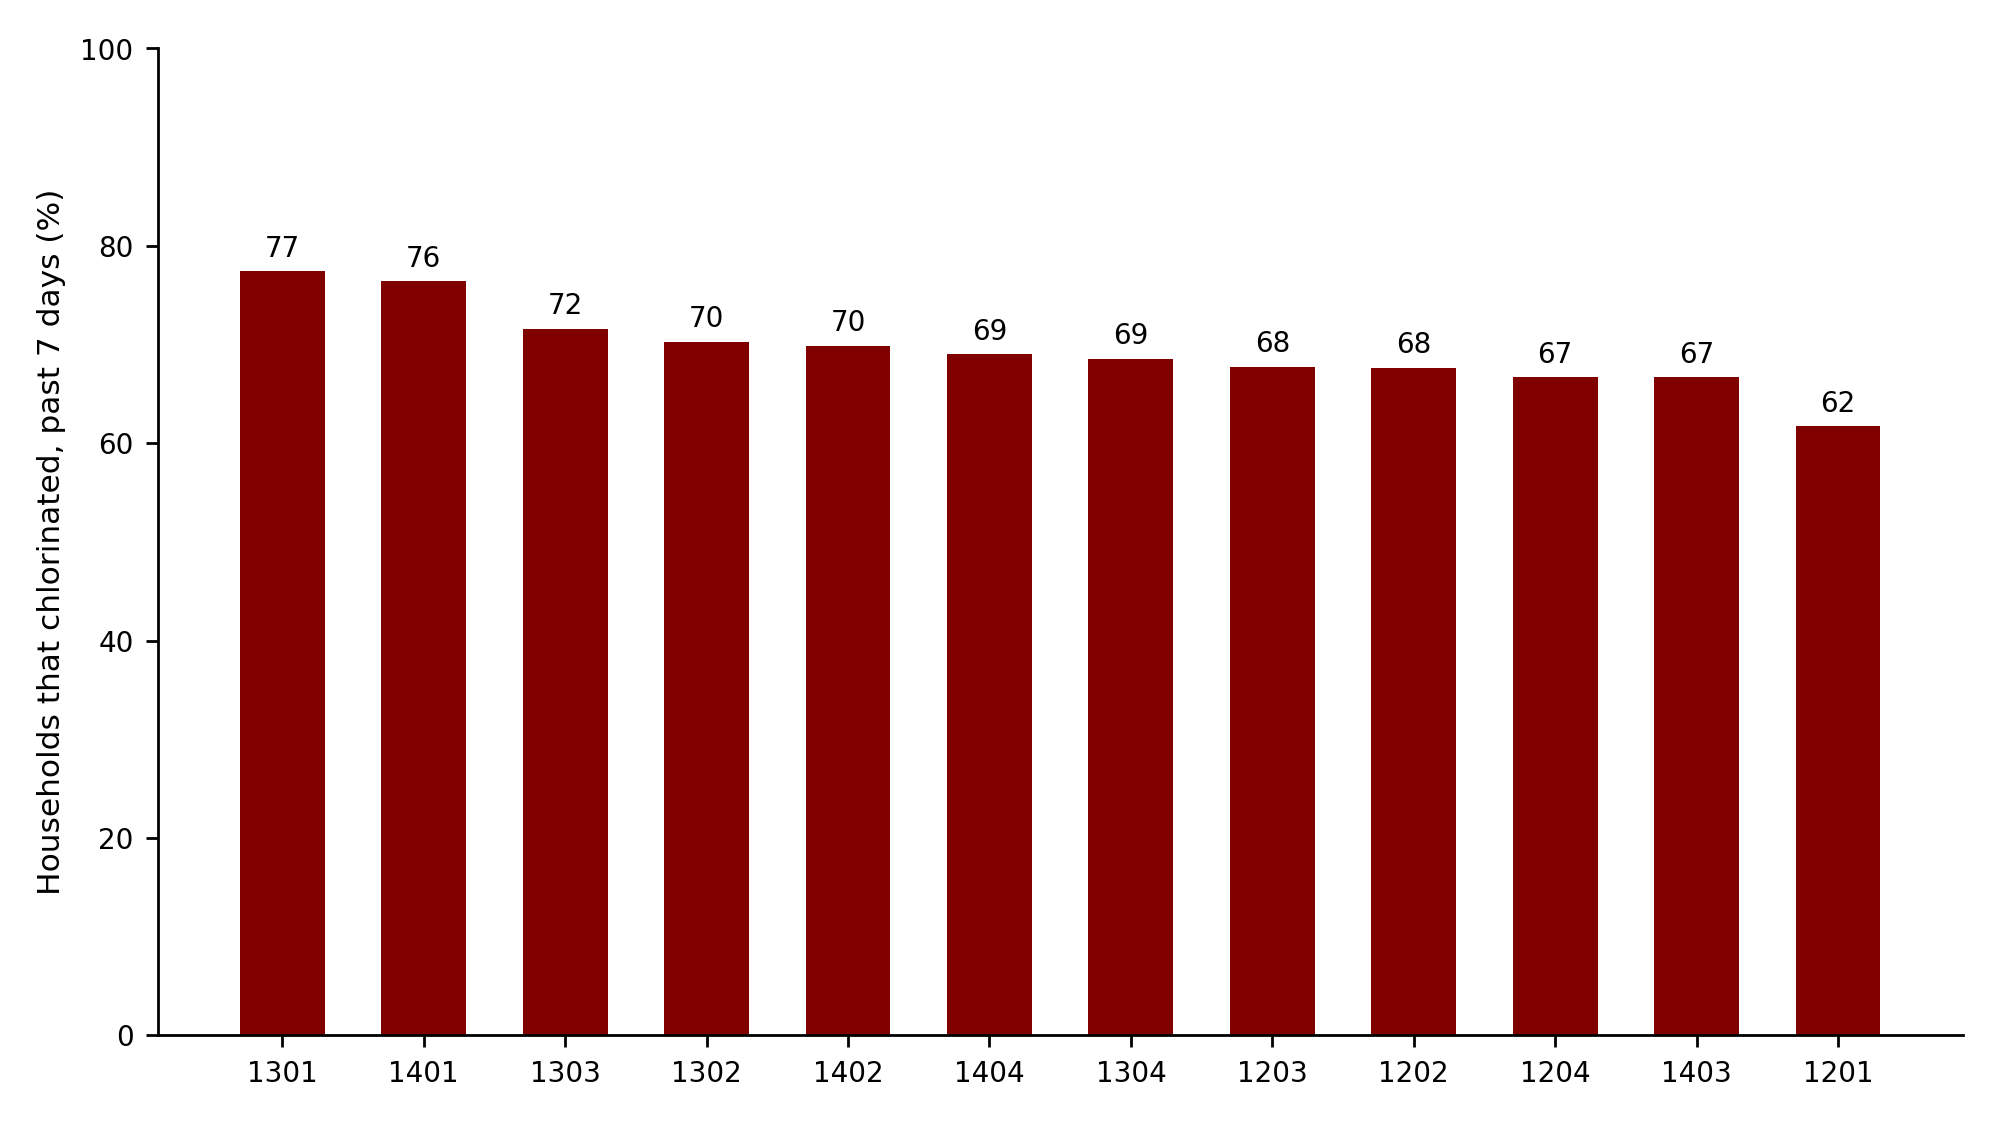
\includegraphics[width=0.85\textwidth]{figures/fig1-chlorination-village.png}
  \caption{Share of households that chlorinated their drinking water in the
    past 7 days, by village. Consenting households, \sampleNote.}
  \label{fig:village}
\end{figure}

\section*{Open questions for the PI}

\begin{enumerate}
  \item Some households report chlorinating or boiling on more than 7 of the
    past 7 days. We exclude those answers from the indicators. Should we?
  \item Some household IDs were submitted twice. They are kept for now,
    pending the high-frequency checks. Should the report use only one visit?
  \item The diarrhea comparison is descriptive. Which controls would you like
    to see before we read anything into it?
\end{enumerate}

\end{document}
